\begin{surferPage}[Çift koni]{Çift koni}
Bu galerinin giriş sayfasında açıklandığı gibi, üstünde (tekillik denen) sivriliklere sahip olmayan
yüzeylere \emph{düzgün} denir; örneğin küre ya da simit (altta en soldaki iki resim):
    \begin{center}
      \begin{tabular}{@{}c@{}c@{}c@{}c@{}}
        \begin{tabular}{@{}c}
          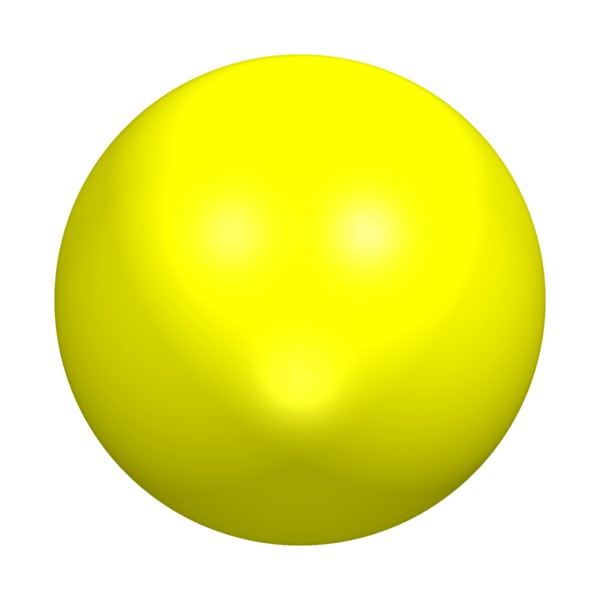
\includegraphics[width=1.4cm]{./../../common/images/kugel}
        \end{tabular}
        &
        \begin{tabular}{@{}c}
          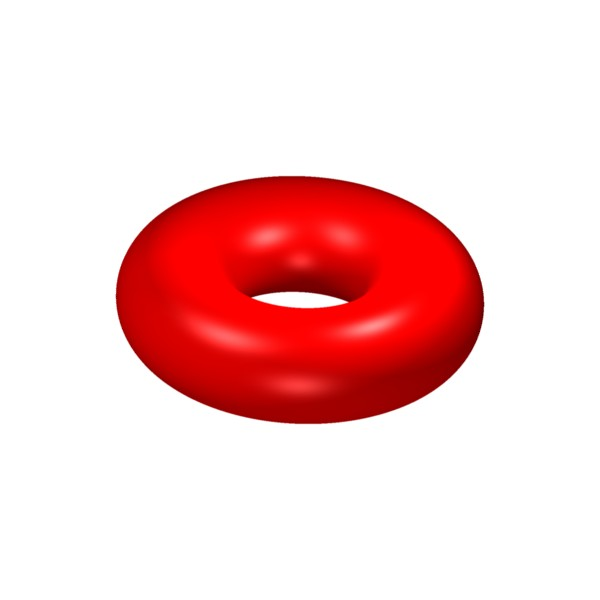
\includegraphics[width=1.4cm]{./../../common/images/torus}
        \end{tabular}
        &
        \begin{tabular}{c@{}}
          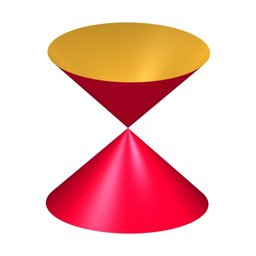
\includegraphics[width=1.4cm]{./../../common/images/kegel}
        \end{tabular}
      \end{tabular}
    \end{center}
Çift koni (en sağdaki resim) en basit tekilliktir; derecesi $2$ olan bir eşitlikle tarif edilebilecek
tek tekilliktir:    
\[x^2+y^2-z^2=0.\]
Bu denklemde $0$'ı çok küçük bir $a\neq 0$ ile yer değiştirince, $a$'nın işaretine bağlı olarak,
çift koni şu iki tür hiperboloidden birine döner:
    \begin{center}
      \begin{tabular}{@{}c@{\ }c@{\ }c@{\ }c@{\ }c@{}}
        \begin{tabular}{@{}c@{}}
          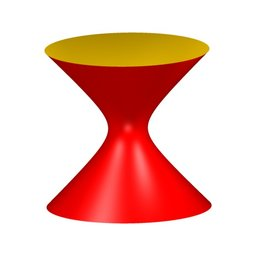
\includegraphics[width=1.2cm]{./../../common/images/A1pm_2}
        \end{tabular}
        &
        $\leftarrow$
        &
        \begin{tabular}{@{}c@{}}
          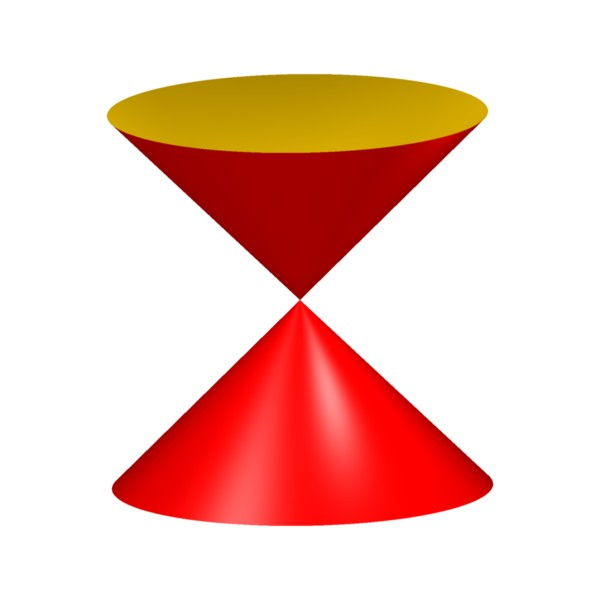
\includegraphics[width=1.2cm]{./../../common/images/A1pm_1} 
        \end{tabular}
        &
        $\rightarrow$
        &
        \begin{tabular}{@{}c@{}}
          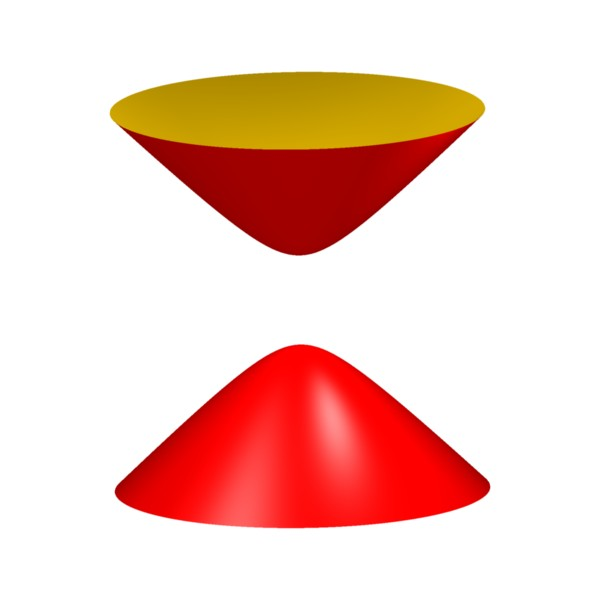
\includegraphics[width=1.2cm]{./../../common/images/A1pm_0}
        \end{tabular}
      \end{tabular}
    \end{center}
   Derecesi $2$  olan bir yüzeyin $1$'den fazla tekilliği olamaz, yani \ $\mu(2)=1$'dir.
\end{surferPage}
